\documentclass[letterpaper,10pt]{book}
% Change to 10 pt
\usepackage{pdfpages}
\usepackage{morewrites}			% to counteract the no write space problem
\setcounter{tocdepth}{5}

\usepackage[framemethod=TikZ]{mdframed}

\usepackage{fancyhdr}

\usepackage{paralist}
\usepackage{amsmath}
\usepackage{amsfonts}
\usepackage{amssymb}
\usepackage{graphicx}

\usepackage{datetime}
%\usepackage{ulem}

%\usepackage[nottoc]{toobibind}

\usepackage[inline]{enumitem}

% Outer margin at 2.50 is exactly correct to fit the ``corruption alert'' tables
\usepackage[inner=1.0in, outer=2.50in, top=2.54cm,bottom=2.54cm, marginparwidth=2.25in]{geometry}

\usepackage{marginnote}
\usepackage{longtable}
\usepackage{booktabs}
\usepackage{xcolor}

\usepackage{soul}

\usepackage{marginnote}
\usepackage{imakeidx} 
\usepackage[
	backref=true,
	style=numeric,
%	citestyle=numeric,
	backend=bibtex
	]{biblatex}
\usepackage[driverfallback=hypertex,colorlinks=True]{hyperref}
\usepackage{cleveref}

\makeindex[name=scripture,columnsep=20pt, columnseprule=True,columns=3, title=Scripture References]
\makeindex[name=speaker,columnsep=20pt, columnseprule=True,,columns=2, title=Sermon Creator]
\makeindex[name=series,columnsep=20pt, columnseprule=True,,columns=2, title=Sermon Series]
\makeindex[name=date,columnsep=20pt, columnseprule=True,columns=2, title=Sermon Date]

\makeindex[name=event,columnsep=20pt, columnseprule=True,columns=2, title=Event]

\makeindex[name=topic,columnsep=20pt, columnseprule=True,columns=2, title=Topic]
\makeindex[name=AWIP,columnsep=20pt, columnseprule=True,columns=3, title=All Words in Passage]
\makeindex[name=NWIV,columnsep=20pt, columnseprule=True,columns=3, title=Number of Words in Verse]
\makeindex[name=PNIP,columnsep=20pt, columnseprule=True,columns=3, title=Proper Names in Passage]
\makeindex[name=PEIP,columnsep=20pt, columnseprule=True,columns=2, title=Prophetic Events in Passage]


\makeindex[name=TWPAQ,columnsep=20pt, columnseprule=True,columns=1, title=13-Word Phrases and Quotes]
\makeindex[name=PFTTIS,columnsep=20pt, columnseprule=False,columns=3, title=Phrases found 13 times in scripture]
\makeindex[name=WFTTIS,columnsep=20pt, columnseprule=False,columns=3, title=Words found 13 times in scripture]
\makeindex[name=WFITV,columnsep=20pt, columnseprule=False,columns=3, title=Words found in exactly 13 verses]
\makeindex[name=EVENTS,columnsep=20pt, columnseprule=False,columns=2, title=Sermon Log by Place]
\makeindex[name=QUESTIONS,columnsep=20pt, columnseprule=False,columns=2, title=Bible Questions]

\makeindex[name=DOCTRINES,columnsep=20pt, columnseprule=False,columns=2, title=Doctrines]

\makeindex[name=SONGS,columnsep=20pt, columnseprule=False,columns=1, title=Songs]
\makeindex[name=LOCATION,columnsep=20pt, columnseprule=False,columns= 2, title=Location]
\makeindex[name=FACEBOOK,columnsep=20pt, columnseprule=False,columns=2, title=Facebook]

\makeindex[name=DEVOTIONAL,columnsep=20pt, columnseprule=False,columns=1, title=Devotionals]

\pagestyle{fancy}
\fancyhf{}
\fancyhead[LE,RO]{\today}
\fancyhead[RE,LO]{Notes, Outlines, Comments}
\fancyhead[CE,CO]{-page \thepage  - }

\fancyfoot[CO,CE]{\leftmark}
%\fancyfoot[LE,RO]{CSCE 692, HW1}

\title{DBR\\
Daily \\ Reads}
\author{Keith Anthony \\
\today }
%\title

%+/ffffff +   \pagenumbering{gobble}

\bibliography{Bibliographies/All20220108}

%%%%% TWEAKS:
%%% - distance from fcolorbox frame to text
\setlength{\fboxsep}{1.0pt}

\usepackage[utf8]{inputenc}
\usepackage{tikz}

%%%%%%%%%%%%%%%%%%%%%%%%%%%%%%%%%%%%%%%%%%%%%%%%%%%%%%%%%%%%%%%%%%%%%%%%%%%%%%%%

\begin{document}

\begin{titlepage}

% Set the text of the page to right-aligned until \end{flushright}
\begin{flushright}
\rightskip=-2.5cm

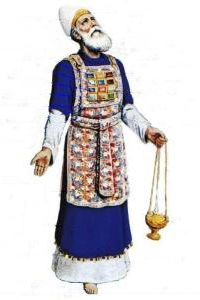
\includegraphics[width=50mm,scale=1.5]{Melchisedec.jpg}
\vspace{0.4in}

% Create a title for the document and write it in bold font
\LARGE{\textbf{\date}}
\linebreak

\vspace{0.5in}


\begin{flushleft}
\LARGE{Hebrews\\}\vspace{0.25in}
\LARGE{Notes, Outlines, Comments}
\end{flushleft}

% write in large letters
%\large{Free webservices and apps}

% Skip some space
\vspace{0.6in}

%\large{Documentation}
% Skip some space

\bigskip

\normalsize{Xenia, Oh.\\}
\normalsize{created: \today}

% Skip some space
\vspace{1.3in}

\end{flushright}
% End the title page
\end{titlepage}

%\titlehttps://www.overleaf.com/project/60d732302fc633866943c9d2JE

\newpage 

\tableofcontents\hypertarget{TOC}{}
\listoffigures
\listoftables

\hyphenation{A-bim-e-lech bre-thren E-phra-im  Gib-e-o-nites Jer-u-sa-lem through-out Phil-i-stines The-o-phil-us Am-a-le-kites ven-geance Mesh-el-e-mi-ah onan-ism Phar-a-oh Py-thon thoughts grev-ous-ness Hach-a-liah adul-ter-er Shad-rach}

%\fcolorbox{black}{bone}{TEXT}
%%%%%%%%%%%%%%%%% EXTRA COLORS
%%%%%%%%%%%%%%%%% EXTRA COLORS
%%%%%%%%%%%%%%%%% EXTRA COLORS
\definecolor{champagne}{rgb}{0.97,0.91,0.81}
\definecolor{bone}{rgb}{0.89,0.85,0.79}

\definecolor{ForestGreen}{rgb}{0.00,0.29,0.098}
\definecolor{GIVING}{cmyk}{1,0.0,0.72,.1}

\definecolor{MLPE}{cmyk}{1,1,0,.45}
\definecolor{SOCCER}{cmyk}{.77, 0, .42, .49}
\definecolor{PAYBILL}{cmyk}{0,0.83,0.76,0.07}
\definecolor{SERMON}{cmyk}{.14,.9,0,.30} % aka seance \href{http://www.flatuicolorpicker.com/purple-cmyk-color-model/}{seance}
\definecolor{BIBLE}{cmyk}{0,.17,.74,.17}
\definecolor{WORKBLUE}{cmyk}{1, .5, 0, .6}
\definecolor{myOrange}{cmyk}{0, .4, .98, .03}
\definecolor{myTan}{cmyk}{0.0,.07,.17,.10}
\definecolor{myRed}{cmyk}{0,1,1,0}
\definecolor{myWhite}{cmyk}{0,0,0,0}
\definecolor{BLUESoD}{cmyk}{.97,.84,0,.04}
\definecolor{WHITE}{cmyk}{0,0,0,0}
\definecolor{OLDGOLD}{cmyk}{0.05,0.3,1.00,0}
\definecolor{CASTLETON}{cmyk}{1,0,0.31,0.66}
\definecolor{cadmiumgreen}{rgb}{0.0, 0.42, 0.24}
\definecolor{jungle}{rgb}{0.203,0.4882,0.1718}
\definecolor{MYGOLD}{rgb}{1,.84,0}

\definecolor{MYLIGHTGRAY}{rgb}{.85,.85,.85}

\definecolor{codegreen}{rgb}{0,0.6,0}
\definecolor{codegray}{rgb}{0.5,0.5,0.5}
\definecolor{codepurple}{rgb}{0.58,0,0.82}
\definecolor{backcolour}{rgb}{0.95,0.95,0.92}



\mdfdefinestyle{MyFrame}{%
    linecolor=blue,
    outerlinewidth=2pt,
    roundcorner=5pt,
    innertopmargin=\baselineskip,
    innerbottommargin=\baselineskip,
    innerrightmargin=10pt,
    innerleftmargin=10pt,
    backgroundcolor=gray!25!white}


\mdfdefinestyle{MyFrame2}{%
    linecolor=black,
    outerlinewidth=2pt,
    roundcorner=5pt,
    innertopmargin=\baselineskip,
    innerbottommargin=\baselineskip,
    innerrightmargin=10pt,
    innerleftmargin=10pt,
    backgroundcolor=yellow!25!white}



%\input{PFTTIS}
%\input{WFTTIS}
%\input{WFITV}


\chapter{Hebrews 4}

\begin{figure}
  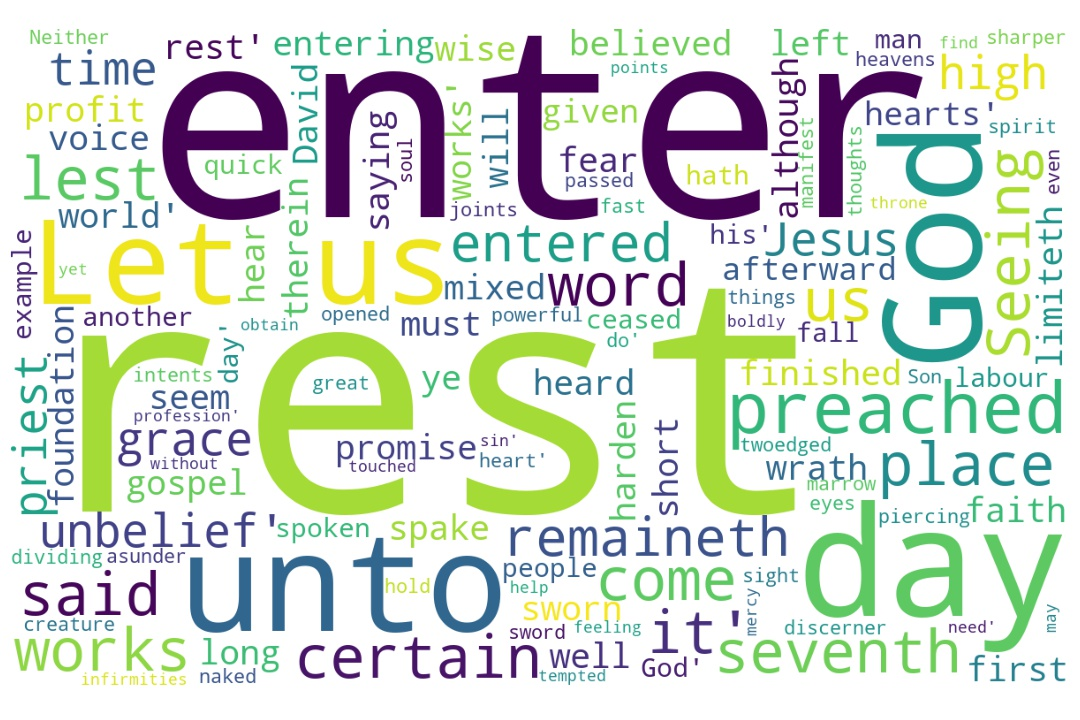
\includegraphics[width=\linewidth]{58NT-Hebrews/Hebrews4-WordCloud.jpg}
  \caption{Hebrews 4 Word Cloud}
  \label{fig:Hebrews 4 Word Cloud}
\end{figure}


\marginpar{\scriptsize \centering \fcolorbox{bone}{lime}{\textbf{A PATH TO REST}}\\ (Hebrews 4:1-16) \begin{compactenum}[I.][8]
    \item Coming \textbf{Short} \index[scripture]{Hebrews!Heb 04:01} (Hebrews 4:1)
    \item Wrath \textbf{Sworn} by God \index[scripture]{Hebrews!Heb 04:03} (Hebrews 4:3)
    \item \textbf{Shown} in Creation \index[scripture]{Hebrews!Heb 04:04} (Hebrews 4:4)
    \item \textbf{Spoken} by David \index[scripture]{Hebrews!Heb 04:07} (Hebrews 4:7) (see Psalm 95)
    \item \textbf{Ceasing} from Works \index[scripture]{Hebrews!Heb 04:10} (Hebrews 4:10)
    \item \textbf{Seeing} the Great High Priest \index[scripture]{Hebrews!Heb 04:14} (Hebrews 4:14)
    \item \textbf{Seeking} Mercy \index[scripture]{Hebrews!Heb 04:16} (Hebrews 4:16)\end{compactenum}}

\marginpar{\scriptsize \centering \fcolorbox{bone}{yellow}{\textbf{AVAILABLE}}\\ (Hebrews 4:1-16) \begin{compactenum}[I.][8]
    \item The \textbf{Promise} \index[scripture]{Hebrews!Heb 04:01} (Hebrews 4:1)
    \item The \textbf{Profit} \index[scripture]{Hebrews!Heb 04:02} (Hebrews 4:2)
    \item The \textbf{Preaching} \index[scripture]{Hebrews!Heb 04:02} (Hebrews 4:2, 6) \index[scripture]{Hebrews!Heb 04:06}
    \item The \textbf{Piercing} \index[scripture]{Hebrews!Heb 04:12} (Hebrews 4:12)
    \item The \textbf{Profit} \index[scripture]{Hebrews!Heb 04:14} (Hebrews 4:14)
\end{compactenum}}
    
% \textcolor[cmyk]{0.99998,1,0,0}{
% \footnote{\textcolor[cmyk]{0.99998,1,0,0}{\hyperlink{TOC}{Return to end of Table of Contents.}}}\footnote{\href{https://www.audioverse.org/english/audiobibles/books/ENGKJV/N/Heb/1}{\textcolor[cmyk]{0.99998,1,0,0}{Hebrews Audio}}}

\footnote{\textcolor[cmyk]{0.99998,1,0,0}{\hyperlink{TOC}{Return to end of Table of Contents.}}}\footnote{\href{https://www.audioverse.org/english/audiobibles/books/ENGKJV/N/Heb/1}{\textcolor[cmyk]{0.99998,1,0,0}{Hebrews Audio}}}\textcolor[cmyk]{0.99998,1,0,0}{Let us therefore fear, lest, a promise being left \emph{us} of entering into his rest, any of you should seem to \fcolorbox{bone}{lime}{come short} of it.}
[2] \textcolor[cmyk]{0.99998,1,0,0}{For unto us was the gospel preached, as well as unto them: but the word preached did not profit them, not being mixed with faith in them that heard \emph{it}.}
[3] \textcolor[cmyk]{0.99998,1,0,0}{For we which have believed do enter into rest, as he said, As I have \fcolorbox{bone}{lime}{sworn in my wrath}, if they shall enter into my rest: although the works were finished from the foundation of the world.}\footnote{\textbf{Psalm 95:11} - Unto whom I sware in my wrath that they should not enter into my rest.} 
[4] \textcolor[cmyk]{0.99998,1,0,0}{For he spake in a certain place of the seventh \emph{day} on this wise, And \fcolorbox{bone}{lime}{God did rest the seventh} \fcolorbox{bone}{lime}{day} from all his works.}\footnote{\textbf{Genesis 2:2} - And on the seventh day God ended his work which he had made; and he rested on the seventh day from all his work which he had made.}\footnote{\textbf{Exodus 20:11} - For in six days the LORD made heaven and earth, the sea, and all that in them is, and rested the seventh day: wherefore the LORD blessed the sabbath day, and hallowed it.}\footnote{\textbf{Exodus 31:17} - It is a sign between me and the children of Israel for ever: for in six days the LORD made heaven and earth, and on the seventh day he rested, and was refreshed.} 
[5] \textcolor[cmyk]{0.99998,1,0,0}{And in this \emph{place} again, If they shall enter into my rest.}
[6] \textcolor[cmyk]{0.99998,1,0,0}{Seeing therefore it remaineth that some must enter therein, and they to whom it was first preached entered not in because of unbelief:}
[7] \textcolor[cmyk]{0.99998,1,0,0}{Again, he limiteth a certain day, \fcolorbox{bone}{lime}{saying in David}, To day, after so long a time; as it is said, To day if ye will hear his voice, harden not your hearts.}\footnote{\textbf{Psalm 95:7} - For he is our God; and we are the people of his pasture, and the sheep of his hand. To day if ye will hear his voice,}
[8] \textcolor[cmyk]{0.99998,1,0,0}{For if Jesus had given them rest, then would he not afterward have spoken of another day.}
[9] \textcolor[cmyk]{0.99998,1,0,0}{There remaineth therefore a rest to the people of God.}\footnote{\textbf{Isaiah 11:10} - And in that day there shall be a root of Jesse, which shall stand for an ensign of the people; to it shall the Gentiles seek: and his rest shall be glorious.}\footnote{\textbf{Ezekiel 34:14} - I will feed them in a good pasture, and upon the high mountains of Israel shall their fold be: there shall they lie in a good fold, and in a fat pasture shall they feed upon the mountains of Israel.}\footnote{\textbf{Zephaniah 3:17} - The LORD thy God in the midst of thee is mighty; he will save, he will rejoice over thee with joy; he will rest in his love, he will joy over thee with singing.} 
[10] \textcolor[cmyk]{0.99998,1,0,0}{For he that is entered into his rest, he also hath \fcolorbox{bone}{lime}{ceased} from his own works, as God \emph{did} from his.}
[11] \textcolor[cmyk]{0.99998,1,0,0}{Let us labour therefore to enter into that rest, lest any man fall after the same example of unbelief.}
[12] \textcolor[cmyk]{0.99998,1,0,0}{For the word of God \emph{is} quick, and powerful, and sharper than any twoedged sword, piercing even to the dividing asunder of soul and spirit, and of the joints and marrow, and \emph{is} a discerner of the thoughts and intents of the heart.}\marginpar{\scriptsize \textcolor[rgb]{0.00,0.545,0.269}{$\rightarrow$ The word of God:
\begin{compactenum}[1.]
	\item is quick (living)
	\item powerful
	\item sharper than any twoedged sword
	\item divides soul \& spirit
	\item discerns the thoughts and intents of the heart
	\item Is given the attributes of God in verse 13 (his), namely, onmiscience
\end{compactenum}}    }
[13] \textcolor[cmyk]{0.99998,1,0,0}{Neither is there any creature that is not manifest in his sight: but all things \emph{are} naked and opened unto the eyes of him with whom we have to do.}
[14] \textcolor[cmyk]{0.99998,1,0,0}{Seeing then that we have a \fcolorbox{bone}{lime}{great high priest}, that is passed into the heavens, Jesus the Son of God, let us hold fast \emph{our} profession.}
[15] \textcolor[cmyk]{0.99998,1,0,0}{For we have not an high priest which cannot be touched with the feeling of our infirmities; but was in all points tempted like as \emph{we} \emph{are,} \emph{yet} without sin.}
[16] \textcolor[cmyk]{0.99998,1,0,0}{Let us therefore come boldly unto the throne of grace, that we may \fcolorbox{bone}{lime}{obtain mercy}, and find grace to help in time of need.}

\section{Hebrews 4 Comments}

\subsection{Numeric Nuggets}
\textbf{13:} The 13$^{th}$ word in the chapter starts the phrase ``into rest.''

\subsection{Hebrews 4 Introduction}

Hebrews 4 is a straightforward passage, made difficult by modern Bible expositors who provide shallow exegesis! For light, the referenced passage is Psalm 95, quoted in verse 7 and referenced  in verse 3. Events referenced are the creation in verse 4, the rebellion on Israel at Kadesh-Barnea in Numbers 13:26-33, and something called a ``rest''. There is also a ``gospel'' that shows up in verse 2.\footnote{\textbf{Numbers 13:26-33} - And they went and came to Moses, and to Aaron, and to all the congregation of the children of Israel, unto the wilderness of Paran, to Kadesh; and brought back word unto them, and unto all the congregation, and shewed them the fruit of the land. [27] And they told him, and said, We came unto the land whither thou sentest us, and surely it floweth with milk and honey; and this is the fruit of it. [28] Nevertheless the people be strong that dwell in the land, and the cities are walled, and very great: and moreover we saw the children of Anak there. [29] The Amalekites dwell in the land of the south: and the Hittites, and the Jebusites, and the Amorites, dwell in the mountains: and the Canaanites dwell by the sea, and by the coast of Jordan. [30] And Caleb stilled the people before Moses, and said, Let us go up at once, and possess it; for we are well able to overcome it. [31] But the men that went up with him said, We be not able to go up against the people; for they are stronger than we. [32] And they brought up an evil report of the land which they had searched unto the children of Israel, saying, The land, through which we have gone to search it, is a land that eateth up the inhabitants thereof; and all the people that we saw in it are men of a great stature. [33] And there we saw the giants, the sons of Anak, which come of the giants: and we were in our own sight as grasshoppers, and so we were in their sight.}

An important distinction to be made, first of all, is between four distinct ``rests'' discussed in Hebrews 3 and 4:
\begin{compactenum}
	\item There is the ``Canaan Rest'' in Hebrews 3:16-19.  Canaan, aka the Promised Land, was available to Israel in Numbers 13, but because of unbelief, they refused to obey God and enter.
	\item There is ``Creation Rest'' in Hebrews 4:3-4, when God rested on the seventh day. Was God tired? Did he need a break? No. This ``sabbath'' rest was a sign to Israel (see Exodus 20:20), and pointed to the Millennium.\footnote{\textbf{Ezekiel 20:20} - And hallow my sabbaths; and they shall be a sign between me and you, that ye may know that I am the LORD your God.}
	\item There is the ``Millennial Rest'' in Hebrews 4:7-8, the 1,000-year reign of Christ on Earth.
	\item There is the ``Believer's Rest'' in Hebrews 4:9-10. 
\end{compactenum}
In Numbers 13 and 14 the Israelites came short of a rest, a the offer was not received with faith,but unbelief.


\subsection{Hebrews 4:2}
Having been accused at times of ``reading things into scripture'', I notice the phenomenon where any time the word ``gospel'' is used in scripture, brethren ``read into'' the word the gospel as found in 1 Corinthians 15:1-4, or better yet, ``read out'' any other possible interpretation.  The word ``gospel'' simply means  ``good news'', and I seriously doubt that Moses was preaching 1 Corinthians 15:1-4 in Numbers 13.  Paul's gospel could not apply in Numbers 13 because it simply was not yet available. What specifically, then, was preached to the Israelites in the wilderness, then? Which gospel is being spoken of here?

As pointed out by a few, the New Testament contains no less than ten separate gospels. The one spoken of here in Hebrews 4:2, is \#8 in the list below:
\begin{compactenum}
	\item The gospel of Matthew
	\item The gospel of Mark
	\item The gospel of Luke
	\item The gospel of John
	\item The gospel of the kingdom
	\item The gospel of the grace of God
	\item The glorious gospel of the blessed God	(also called ``my gospel'' by Paul).\footnote{\textbf{Romans 2:16} - In the day when God shall judge the secrets of men by Jesus Christ according to my gospel.}\footnote{\textbf{1 Timothy 1:11} - According to the glorious gospel of the blessed God, which was committed to my trust.}
	\item The gospel of military conflict preached to the nation of Israel: God would give them victory in the military conquest of the land of Canaan to the extent that they obeyed Him (Numbers 13:30, 14:6-10, Hebrews 4:2). \footnote{\textbf{Numbers 14:6-10} - And Joshua the son of Nun, and Caleb the son of Jephunneh, which were of them that searched the land, rent their clothes: [7] And they spake unto all the company of the children of Israel, saying, The land, which we passed through to search it, is an exceeding good land. [8] If the LORD delight in us, then he will bring us into this land, and give it us; a land which floweth with milk and honey. [9] Only rebel not ye against the LORD, neither fear ye the people of the land; for they are bread for us: their defence is departed from them, and the LORD is with us: fear them not. [10] But all the congregation bade stone them with stones. And the glory of the LORD appeared in the tabernacle of the congregation before all the children of Israel.}
	\item The gospel preached to the saints in paradise.\footnote{\textbf{1 Peter 4:6} - For for this cause was the gospel preached also to them that are dead, that they might be judged according to men in the flesh, but live according to God in the spirit.}
	\item The everlasting gospel.\footnote{\textbf{Revelation 14:6} - And I saw another angel fly in the midst of heaven, having the everlasting gospel to preach unto them that dwell on the earth, and to every nation, and kindred, and tongue, and people,}
\end{compactenum}

\subsection{Hebrews 4:4}
See 2 Peter 3:8-10 and the 7$^{th}$ day of creation.\footnote{\textbf{2 Peter 3:8-10} - But, beloved, be not ignorant of this one thing, that one day is with the Lord as a thousand years, and a thousand years as one day. [9] The Lord is not slack concerning his promise, as some men count slackness; but is longsuffering to us-ward, not willing that any should perish, but that all should come to repentance. [10] But the day of the Lord will come as a thief in the night; in the which the heavens shall pass away with a great noise, and the elements shall melt with fervent heat, the earth also and the works that are therein shall be burned up.} 

\subsection{Hebrews 4:8}
Jesus here is speaking of Joshua.

\subsection{Hebrews 4:12}
stuff.%\footnote{}

\subsection{Hebrews 4:15}
This is empathy.

%\index[NWIV]{25!Hebrews!Heb 4:1}\index[AWIP]{Let!Hebrews!Heb 4:1}\index[AWIP]{us!Hebrews!Heb 4:1}\index[AWIP]{therefore!Hebrews!Heb 4:1}\index[AWIP]{fear!Hebrews!Heb 4:1}\index[AWIP]{lest!Hebrews!Heb 4:1}\index[AWIP]{a!Hebrews!Heb 4:1}\index[AWIP]{promise!Hebrews!Heb 4:1}\index[AWIP]{being!Hebrews!Heb 4:1}\index[AWIP]{left!Hebrews!Heb 4:1}\index[AWIP]{\emph{us}!Hebrews!Heb 4:1}\index[AWIP]{of!Hebrews!Heb 4:1}\index[AWIP]{of!Hebrews!Heb 4:1 (2)}\index[AWIP]{of!Hebrews!Heb 4:1 (3)}\index[AWIP]{entering!Hebrews!Heb 4:1}\index[AWIP]{into!Hebrews!Heb 4:1}\index[AWIP]{his!Hebrews!Heb 4:1}\index[AWIP]{rest!Hebrews!Heb 4:1}\index[AWIP]{any!Hebrews!Heb 4:1}\index[AWIP]{you!Hebrews!Heb 4:1}\index[AWIP]{should!Hebrews!Heb 4:1}\index[AWIP]{seem!Hebrews!Heb 4:1}\index[AWIP]{to!Hebrews!Heb 4:1}\index[AWIP]{come!Hebrews!Heb 4:1}\index[AWIP]{short!Hebrews!Heb 4:1}\index[AWIP]{it!Hebrews!Heb 4:1}\index[AWIP]{\emph{us}!Hebrews!Heb 4:1}

\index[NWIV]{30!Hebrews!Heb 4:2}\index[AWIP]{For!Hebrews!Heb 4:2}\index[AWIP]{unto!Hebrews!Heb 4:2}\index[AWIP]{unto!Hebrews!Heb 4:2 (2)}\index[AWIP]{us!Hebrews!Heb 4:2}\index[AWIP]{was!Hebrews!Heb 4:2}\index[AWIP]{the!Hebrews!Heb 4:2}\index[AWIP]{the!Hebrews!Heb 4:2 (2)}\index[AWIP]{gospel!Hebrews!Heb 4:2}\index[AWIP]{preached!Hebrews!Heb 4:2}\index[AWIP]{preached!Hebrews!Heb 4:2 (2)}\index[AWIP]{as!Hebrews!Heb 4:2}\index[AWIP]{as!Hebrews!Heb 4:2 (2)}\index[AWIP]{well!Hebrews!Heb 4:2}\index[AWIP]{them!Hebrews!Heb 4:2}\index[AWIP]{them!Hebrews!Heb 4:2 (2)}\index[AWIP]{them!Hebrews!Heb 4:2 (3)}\index[AWIP]{but!Hebrews!Heb 4:2}\index[AWIP]{word!Hebrews!Heb 4:2}\index[AWIP]{did!Hebrews!Heb 4:2}\index[AWIP]{not!Hebrews!Heb 4:2}\index[AWIP]{not!Hebrews!Heb 4:2 (2)}\index[AWIP]{profit!Hebrews!Heb 4:2}\index[AWIP]{being!Hebrews!Heb 4:2}\index[AWIP]{mixed!Hebrews!Heb 4:2}\index[AWIP]{with!Hebrews!Heb 4:2}\index[AWIP]{faith!Hebrews!Heb 4:2}\index[AWIP]{in!Hebrews!Heb 4:2}\index[AWIP]{that!Hebrews!Heb 4:2}\index[AWIP]{heard!Hebrews!Heb 4:2}\index[AWIP]{\emph{it}!Hebrews!Heb 4:2}\index[AWIP]{\emph{it}!Hebrews!Heb 4:2}

\index[NWIV]{37!Hebrews!Heb 4:3}\index[AWIP]{For!Hebrews!Heb 4:3}\index[AWIP]{we!Hebrews!Heb 4:3}\index[AWIP]{which!Hebrews!Heb 4:3}\index[AWIP]{have!Hebrews!Heb 4:3}\index[AWIP]{have!Hebrews!Heb 4:3 (2)}\index[AWIP]{believed!Hebrews!Heb 4:3}\index[AWIP]{do!Hebrews!Heb 4:3}\index[AWIP]{enter!Hebrews!Heb 4:3}\index[AWIP]{enter!Hebrews!Heb 4:3 (2)}\index[AWIP]{into!Hebrews!Heb 4:3}\index[AWIP]{into!Hebrews!Heb 4:3 (2)}\index[AWIP]{rest!Hebrews!Heb 4:3}\index[AWIP]{rest!Hebrews!Heb 4:3 (2)}\index[AWIP]{as!Hebrews!Heb 4:3}\index[AWIP]{he!Hebrews!Heb 4:3}\index[AWIP]{said!Hebrews!Heb 4:3}\index[AWIP]{As!Hebrews!Heb 4:3}\index[AWIP]{I!Hebrews!Heb 4:3}\index[AWIP]{sworn!Hebrews!Heb 4:3}\index[AWIP]{in!Hebrews!Heb 4:3}\index[AWIP]{my!Hebrews!Heb 4:3}\index[AWIP]{my!Hebrews!Heb 4:3 (2)}\index[AWIP]{wrath!Hebrews!Heb 4:3}\index[AWIP]{if!Hebrews!Heb 4:3}\index[AWIP]{they!Hebrews!Heb 4:3}\index[AWIP]{shall!Hebrews!Heb 4:3}\index[AWIP]{although!Hebrews!Heb 4:3}\index[AWIP]{the!Hebrews!Heb 4:3}\index[AWIP]{the!Hebrews!Heb 4:3 (2)}\index[AWIP]{the!Hebrews!Heb 4:3 (3)}\index[AWIP]{works!Hebrews!Heb 4:3}\index[AWIP]{were!Hebrews!Heb 4:3}\index[AWIP]{finished!Hebrews!Heb 4:3}\index[AWIP]{from!Hebrews!Heb 4:3}\index[AWIP]{foundation!Hebrews!Heb 4:3}\index[AWIP]{of!Hebrews!Heb 4:3}\index[AWIP]{world!Hebrews!Heb 4:3}

\index[NWIV]{25!Hebrews!Heb 4:4}\index[AWIP]{For!Hebrews!Heb 4:4}\index[AWIP]{he!Hebrews!Heb 4:4}\index[AWIP]{spake!Hebrews!Heb 4:4}\index[AWIP]{in!Hebrews!Heb 4:4}\index[AWIP]{a!Hebrews!Heb 4:4}\index[AWIP]{certain!Hebrews!Heb 4:4}\index[AWIP]{place!Hebrews!Heb 4:4}\index[AWIP]{of!Hebrews!Heb 4:4}\index[AWIP]{the!Hebrews!Heb 4:4}\index[AWIP]{the!Hebrews!Heb 4:4 (2)}\index[AWIP]{seventh!Hebrews!Heb 4:4}\index[AWIP]{seventh!Hebrews!Heb 4:4 (2)}\index[AWIP]{\emph{day}!Hebrews!Heb 4:4}\index[AWIP]{on!Hebrews!Heb 4:4}\index[AWIP]{this!Hebrews!Heb 4:4}\index[AWIP]{wise!Hebrews!Heb 4:4}\index[AWIP]{And!Hebrews!Heb 4:4}\index[AWIP]{God!Hebrews!Heb 4:4}\index[AWIP]{did!Hebrews!Heb 4:4}\index[AWIP]{rest!Hebrews!Heb 4:4}\index[AWIP]{day!Hebrews!Heb 4:4}\index[AWIP]{from!Hebrews!Heb 4:4}\index[AWIP]{all!Hebrews!Heb 4:4}\index[AWIP]{his!Hebrews!Heb 4:4}\index[AWIP]{works!Hebrews!Heb 4:4}\index[AWIP]{\emph{day}!Hebrews!Heb 4:4}

\index[NWIV]{12!Hebrews!Heb 4:5}\index[AWIP]{And!Hebrews!Heb 4:5}\index[AWIP]{in!Hebrews!Heb 4:5}\index[AWIP]{this!Hebrews!Heb 4:5}\index[AWIP]{\emph{place}!Hebrews!Heb 4:5}\index[AWIP]{again!Hebrews!Heb 4:5}\index[AWIP]{If!Hebrews!Heb 4:5}\index[AWIP]{they!Hebrews!Heb 4:5}\index[AWIP]{shall!Hebrews!Heb 4:5}\index[AWIP]{enter!Hebrews!Heb 4:5}\index[AWIP]{into!Hebrews!Heb 4:5}\index[AWIP]{my!Hebrews!Heb 4:5}\index[AWIP]{rest!Hebrews!Heb 4:5}\index[AWIP]{\emph{place}!Hebrews!Heb 4:5}

\index[NWIV]{23!Hebrews!Heb 4:6}\index[AWIP]{Seeing!Hebrews!Heb 4:6}\index[AWIP]{therefore!Hebrews!Heb 4:6}\index[AWIP]{it!Hebrews!Heb 4:6}\index[AWIP]{it!Hebrews!Heb 4:6 (2)}\index[AWIP]{remaineth!Hebrews!Heb 4:6}\index[AWIP]{that!Hebrews!Heb 4:6}\index[AWIP]{some!Hebrews!Heb 4:6}\index[AWIP]{must!Hebrews!Heb 4:6}\index[AWIP]{enter!Hebrews!Heb 4:6}\index[AWIP]{therein!Hebrews!Heb 4:6}\index[AWIP]{and!Hebrews!Heb 4:6}\index[AWIP]{they!Hebrews!Heb 4:6}\index[AWIP]{to!Hebrews!Heb 4:6}\index[AWIP]{whom!Hebrews!Heb 4:6}\index[AWIP]{was!Hebrews!Heb 4:6}\index[AWIP]{first!Hebrews!Heb 4:6}\index[AWIP]{preached!Hebrews!Heb 4:6}\index[AWIP]{entered!Hebrews!Heb 4:6}\index[AWIP]{not!Hebrews!Heb 4:6}\index[AWIP]{in!Hebrews!Heb 4:6}\index[AWIP]{because!Hebrews!Heb 4:6}\index[AWIP]{of!Hebrews!Heb 4:6}\index[AWIP]{unbelief!Hebrews!Heb 4:6}

\index[NWIV]{32!Hebrews!Heb 4:7}\index[AWIP]{Again!Hebrews!Heb 4:7}\index[AWIP]{he!Hebrews!Heb 4:7}\index[AWIP]{limiteth!Hebrews!Heb 4:7}\index[AWIP]{a!Hebrews!Heb 4:7}\index[AWIP]{a!Hebrews!Heb 4:7 (2)}\index[AWIP]{certain!Hebrews!Heb 4:7}\index[AWIP]{day!Hebrews!Heb 4:7}\index[AWIP]{day!Hebrews!Heb 4:7 (2)}\index[AWIP]{day!Hebrews!Heb 4:7 (3)}\index[AWIP]{saying!Hebrews!Heb 4:7}\index[AWIP]{in!Hebrews!Heb 4:7}\index[AWIP]{David!Hebrews!Heb 4:7}\index[AWIP]{To!Hebrews!Heb 4:7}\index[AWIP]{To!Hebrews!Heb 4:7 (2)}\index[AWIP]{after!Hebrews!Heb 4:7}\index[AWIP]{so!Hebrews!Heb 4:7}\index[AWIP]{long!Hebrews!Heb 4:7}\index[AWIP]{time!Hebrews!Heb 4:7}\index[AWIP]{as!Hebrews!Heb 4:7}\index[AWIP]{it!Hebrews!Heb 4:7}\index[AWIP]{is!Hebrews!Heb 4:7}\index[AWIP]{said!Hebrews!Heb 4:7}\index[AWIP]{if!Hebrews!Heb 4:7}\index[AWIP]{ye!Hebrews!Heb 4:7}\index[AWIP]{will!Hebrews!Heb 4:7}\index[AWIP]{hear!Hebrews!Heb 4:7}\index[AWIP]{his!Hebrews!Heb 4:7}\index[AWIP]{voice!Hebrews!Heb 4:7}\index[AWIP]{harden!Hebrews!Heb 4:7}\index[AWIP]{not!Hebrews!Heb 4:7}\index[AWIP]{your!Hebrews!Heb 4:7}\index[AWIP]{hearts!Hebrews!Heb 4:7}

\index[NWIV]{17!Hebrews!Heb 4:8}\index[AWIP]{For!Hebrews!Heb 4:8}\index[AWIP]{if!Hebrews!Heb 4:8}\index[AWIP]{Jesus!Hebrews!Heb 4:8}\index[AWIP]{had!Hebrews!Heb 4:8}\index[AWIP]{given!Hebrews!Heb 4:8}\index[AWIP]{them!Hebrews!Heb 4:8}\index[AWIP]{rest!Hebrews!Heb 4:8}\index[AWIP]{then!Hebrews!Heb 4:8}\index[AWIP]{would!Hebrews!Heb 4:8}\index[AWIP]{he!Hebrews!Heb 4:8}\index[AWIP]{not!Hebrews!Heb 4:8}\index[AWIP]{afterward!Hebrews!Heb 4:8}\index[AWIP]{have!Hebrews!Heb 4:8}\index[AWIP]{spoken!Hebrews!Heb 4:8}\index[AWIP]{of!Hebrews!Heb 4:8}\index[AWIP]{another!Hebrews!Heb 4:8}\index[AWIP]{day!Hebrews!Heb 4:8}

\index[NWIV]{10!Hebrews!Heb 4:9}\index[AWIP]{There!Hebrews!Heb 4:9}\index[AWIP]{remaineth!Hebrews!Heb 4:9}\index[AWIP]{therefore!Hebrews!Heb 4:9}\index[AWIP]{a!Hebrews!Heb 4:9}\index[AWIP]{rest!Hebrews!Heb 4:9}\index[AWIP]{to!Hebrews!Heb 4:9}\index[AWIP]{the!Hebrews!Heb 4:9}\index[AWIP]{people!Hebrews!Heb 4:9}\index[AWIP]{of!Hebrews!Heb 4:9}\index[AWIP]{God!Hebrews!Heb 4:9}

\index[NWIV]{21!Hebrews!Heb 4:10}\index[AWIP]{For!Hebrews!Heb 4:10}\index[AWIP]{he!Hebrews!Heb 4:10}\index[AWIP]{he!Hebrews!Heb 4:10 (2)}\index[AWIP]{that!Hebrews!Heb 4:10}\index[AWIP]{is!Hebrews!Heb 4:10}\index[AWIP]{entered!Hebrews!Heb 4:10}\index[AWIP]{into!Hebrews!Heb 4:10}\index[AWIP]{his!Hebrews!Heb 4:10}\index[AWIP]{his!Hebrews!Heb 4:10 (2)}\index[AWIP]{his!Hebrews!Heb 4:10 (3)}\index[AWIP]{rest!Hebrews!Heb 4:10}\index[AWIP]{also!Hebrews!Heb 4:10}\index[AWIP]{hath!Hebrews!Heb 4:10}\index[AWIP]{ceased!Hebrews!Heb 4:10}\index[AWIP]{from!Hebrews!Heb 4:10}\index[AWIP]{from!Hebrews!Heb 4:10 (2)}\index[AWIP]{own!Hebrews!Heb 4:10}\index[AWIP]{works!Hebrews!Heb 4:10}\index[AWIP]{as!Hebrews!Heb 4:10}\index[AWIP]{God!Hebrews!Heb 4:10}\index[AWIP]{\emph{did}!Hebrews!Heb 4:10}\index[AWIP]{\emph{did}!Hebrews!Heb 4:10}

\index[NWIV]{19!Hebrews!Heb 4:11}\index[AWIP]{Let!Hebrews!Heb 4:11}\index[AWIP]{us!Hebrews!Heb 4:11}\index[AWIP]{labour!Hebrews!Heb 4:11}\index[AWIP]{therefore!Hebrews!Heb 4:11}\index[AWIP]{to!Hebrews!Heb 4:11}\index[AWIP]{enter!Hebrews!Heb 4:11}\index[AWIP]{into!Hebrews!Heb 4:11}\index[AWIP]{that!Hebrews!Heb 4:11}\index[AWIP]{rest!Hebrews!Heb 4:11}\index[AWIP]{lest!Hebrews!Heb 4:11}\index[AWIP]{any!Hebrews!Heb 4:11}\index[AWIP]{man!Hebrews!Heb 4:11}\index[AWIP]{fall!Hebrews!Heb 4:11}\index[AWIP]{after!Hebrews!Heb 4:11}\index[AWIP]{the!Hebrews!Heb 4:11}\index[AWIP]{same!Hebrews!Heb 4:11}\index[AWIP]{example!Hebrews!Heb 4:11}\index[AWIP]{of!Hebrews!Heb 4:11}\index[AWIP]{unbelief!Hebrews!Heb 4:11}

\index[NWIV]{43!Hebrews!Heb 4:12}\index[AWIP]{For!Hebrews!Heb 4:12}\index[AWIP]{the!Hebrews!Heb 4:12}\index[AWIP]{the!Hebrews!Heb 4:12 (2)}\index[AWIP]{the!Hebrews!Heb 4:12 (3)}\index[AWIP]{the!Hebrews!Heb 4:12 (4)}\index[AWIP]{the!Hebrews!Heb 4:12 (5)}\index[AWIP]{word!Hebrews!Heb 4:12}\index[AWIP]{of!Hebrews!Heb 4:12}\index[AWIP]{of!Hebrews!Heb 4:12 (2)}\index[AWIP]{of!Hebrews!Heb 4:12 (3)}\index[AWIP]{of!Hebrews!Heb 4:12 (4)}\index[AWIP]{of!Hebrews!Heb 4:12 (5)}\index[AWIP]{God!Hebrews!Heb 4:12}\index[AWIP]{\emph{is}!Hebrews!Heb 4:12}\index[AWIP]{\emph{is}!Hebrews!Heb 4:12 (2)}\index[AWIP]{quick!Hebrews!Heb 4:12}\index[AWIP]{and!Hebrews!Heb 4:12}\index[AWIP]{and!Hebrews!Heb 4:12 (2)}\index[AWIP]{and!Hebrews!Heb 4:12 (3)}\index[AWIP]{and!Hebrews!Heb 4:12 (4)}\index[AWIP]{and!Hebrews!Heb 4:12 (5)}\index[AWIP]{and!Hebrews!Heb 4:12 (6)}\index[AWIP]{and!Hebrews!Heb 4:12 (7)}\index[AWIP]{powerful!Hebrews!Heb 4:12}\index[AWIP]{sharper!Hebrews!Heb 4:12}\index[AWIP]{than!Hebrews!Heb 4:12}\index[AWIP]{any!Hebrews!Heb 4:12}\index[AWIP]{twoedged!Hebrews!Heb 4:12}\index[AWIP]{sword!Hebrews!Heb 4:12}\index[AWIP]{piercing!Hebrews!Heb 4:12}\index[AWIP]{even!Hebrews!Heb 4:12}\index[AWIP]{to!Hebrews!Heb 4:12}\index[AWIP]{dividing!Hebrews!Heb 4:12}\index[AWIP]{asunder!Hebrews!Heb 4:12}\index[AWIP]{soul!Hebrews!Heb 4:12}\index[AWIP]{spirit!Hebrews!Heb 4:12}\index[AWIP]{joints!Hebrews!Heb 4:12}\index[AWIP]{marrow!Hebrews!Heb 4:12}\index[AWIP]{a!Hebrews!Heb 4:12}\index[AWIP]{discerner!Hebrews!Heb 4:12}\index[AWIP]{thoughts!Hebrews!Heb 4:12}\index[AWIP]{intents!Hebrews!Heb 4:12}\index[AWIP]{heart!Hebrews!Heb 4:12}\index[AWIP]{\emph{is}!Hebrews!Heb 4:12}\index[AWIP]{\emph{is}!Hebrews!Heb 4:12 (2)}

\index[NWIV]{30!Hebrews!Heb 4:13}\index[AWIP]{Neither!Hebrews!Heb 4:13}\index[AWIP]{is!Hebrews!Heb 4:13}\index[AWIP]{is!Hebrews!Heb 4:13 (2)}\index[AWIP]{there!Hebrews!Heb 4:13}\index[AWIP]{any!Hebrews!Heb 4:13}\index[AWIP]{creature!Hebrews!Heb 4:13}\index[AWIP]{that!Hebrews!Heb 4:13}\index[AWIP]{not!Hebrews!Heb 4:13}\index[AWIP]{manifest!Hebrews!Heb 4:13}\index[AWIP]{in!Hebrews!Heb 4:13}\index[AWIP]{his!Hebrews!Heb 4:13}\index[AWIP]{sight!Hebrews!Heb 4:13}\index[AWIP]{but!Hebrews!Heb 4:13}\index[AWIP]{all!Hebrews!Heb 4:13}\index[AWIP]{things!Hebrews!Heb 4:13}\index[AWIP]{\emph{are}!Hebrews!Heb 4:13}\index[AWIP]{naked!Hebrews!Heb 4:13}\index[AWIP]{and!Hebrews!Heb 4:13}\index[AWIP]{opened!Hebrews!Heb 4:13}\index[AWIP]{unto!Hebrews!Heb 4:13}\index[AWIP]{the!Hebrews!Heb 4:13}\index[AWIP]{eyes!Hebrews!Heb 4:13}\index[AWIP]{of!Hebrews!Heb 4:13}\index[AWIP]{him!Hebrews!Heb 4:13}\index[AWIP]{with!Hebrews!Heb 4:13}\index[AWIP]{whom!Hebrews!Heb 4:13}\index[AWIP]{we!Hebrews!Heb 4:13}\index[AWIP]{have!Hebrews!Heb 4:13}\index[AWIP]{to!Hebrews!Heb 4:13}\index[AWIP]{do!Hebrews!Heb 4:13}\index[AWIP]{\emph{are}!Hebrews!Heb 4:13}

\index[NWIV]{26!Hebrews!Heb 4:14}\index[AWIP]{Seeing!Hebrews!Heb 4:14}\index[AWIP]{then!Hebrews!Heb 4:14}\index[AWIP]{that!Hebrews!Heb 4:14}\index[AWIP]{that!Hebrews!Heb 4:14 (2)}\index[AWIP]{we!Hebrews!Heb 4:14}\index[AWIP]{have!Hebrews!Heb 4:14}\index[AWIP]{a!Hebrews!Heb 4:14}\index[AWIP]{great!Hebrews!Heb 4:14}\index[AWIP]{high!Hebrews!Heb 4:14}\index[AWIP]{priest!Hebrews!Heb 4:14}\index[AWIP]{is!Hebrews!Heb 4:14}\index[AWIP]{passed!Hebrews!Heb 4:14}\index[AWIP]{into!Hebrews!Heb 4:14}\index[AWIP]{the!Hebrews!Heb 4:14}\index[AWIP]{the!Hebrews!Heb 4:14 (2)}\index[AWIP]{heavens!Hebrews!Heb 4:14}\index[AWIP]{Jesus!Hebrews!Heb 4:14}\index[AWIP]{Son!Hebrews!Heb 4:14}\index[AWIP]{of!Hebrews!Heb 4:14}\index[AWIP]{God!Hebrews!Heb 4:14}\index[AWIP]{let!Hebrews!Heb 4:14}\index[AWIP]{us!Hebrews!Heb 4:14}\index[AWIP]{hold!Hebrews!Heb 4:14}\index[AWIP]{fast!Hebrews!Heb 4:14}\index[AWIP]{\emph{our}!Hebrews!Heb 4:14}\index[AWIP]{profession!Hebrews!Heb 4:14}\index[AWIP]{\emph{our}!Hebrews!Heb 4:14}

\index[NWIV]{30!Hebrews!Heb 4:15}\index[AWIP]{For!Hebrews!Heb 4:15}\index[AWIP]{we!Hebrews!Heb 4:15}\index[AWIP]{have!Hebrews!Heb 4:15}\index[AWIP]{not!Hebrews!Heb 4:15}\index[AWIP]{an!Hebrews!Heb 4:15}\index[AWIP]{high!Hebrews!Heb 4:15}\index[AWIP]{priest!Hebrews!Heb 4:15}\index[AWIP]{which!Hebrews!Heb 4:15}\index[AWIP]{cannot!Hebrews!Heb 4:15}\index[AWIP]{be!Hebrews!Heb 4:15}\index[AWIP]{touched!Hebrews!Heb 4:15}\index[AWIP]{with!Hebrews!Heb 4:15}\index[AWIP]{the!Hebrews!Heb 4:15}\index[AWIP]{feeling!Hebrews!Heb 4:15}\index[AWIP]{of!Hebrews!Heb 4:15}\index[AWIP]{our!Hebrews!Heb 4:15}\index[AWIP]{infirmities!Hebrews!Heb 4:15}\index[AWIP]{but!Hebrews!Heb 4:15}\index[AWIP]{was!Hebrews!Heb 4:15}\index[AWIP]{in!Hebrews!Heb 4:15}\index[AWIP]{all!Hebrews!Heb 4:15}\index[AWIP]{points!Hebrews!Heb 4:15}\index[AWIP]{tempted!Hebrews!Heb 4:15}\index[AWIP]{like!Hebrews!Heb 4:15}\index[AWIP]{as!Hebrews!Heb 4:15}\index[AWIP]{\emph{we}!Hebrews!Heb 4:15}\index[AWIP]{\emph{are}!Hebrews!Heb 4:15}\index[AWIP]{\emph{yet}!Hebrews!Heb 4:15}\index[AWIP]{without!Hebrews!Heb 4:15}\index[AWIP]{sin!Hebrews!Heb 4:15}\index[AWIP]{\emph{we}!Hebrews!Heb 4:15}\index[AWIP]{\emph{are}!Hebrews!Heb 4:15}\index[AWIP]{\emph{yet}!Hebrews!Heb 4:15}

\index[NWIV]{24!Hebrews!Heb 4:16}\index[AWIP]{Let!Hebrews!Heb 4:16}\index[AWIP]{us!Hebrews!Heb 4:16}\index[AWIP]{therefore!Hebrews!Heb 4:16}\index[AWIP]{come!Hebrews!Heb 4:16}\index[AWIP]{boldly!Hebrews!Heb 4:16}\index[AWIP]{unto!Hebrews!Heb 4:16}\index[AWIP]{the!Hebrews!Heb 4:16}\index[AWIP]{throne!Hebrews!Heb 4:16}\index[AWIP]{of!Hebrews!Heb 4:16}\index[AWIP]{of!Hebrews!Heb 4:16 (2)}\index[AWIP]{grace!Hebrews!Heb 4:16}\index[AWIP]{grace!Hebrews!Heb 4:16 (2)}\index[AWIP]{that!Hebrews!Heb 4:16}\index[AWIP]{we!Hebrews!Heb 4:16}\index[AWIP]{may!Hebrews!Heb 4:16}\index[AWIP]{obtain!Hebrews!Heb 4:16}\index[AWIP]{mercy!Hebrews!Heb 4:16}\index[AWIP]{and!Hebrews!Heb 4:16}\index[AWIP]{find!Hebrews!Heb 4:16}\index[AWIP]{to!Hebrews!Heb 4:16}\index[AWIP]{help!Hebrews!Heb 4:16}\index[AWIP]{in!Hebrews!Heb 4:16}\index[AWIP]{time!Hebrews!Heb 4:16}\index[AWIP]{need!Hebrews!Heb 4:16}


\section{Hebrews 4 Outlines}

\subsection{My Outlines}


\subsubsection{A Path to Rest}
\index[speaker]{Keith Anthony!Hebrews 04 (A Path to Rest)}
\index[series]{Hebrews (Keith Anthony)!Hebrews 04 (A Path to Rest)}
\index[date]{2016/12/06!Hebrews 04 (A Path to Rest) (Keith Anthony)}
%\textbf{Introduction:} Paul has good words for their:
\begin{compactenum}[I.][8]
    \item Coming \textbf{Short} \index[scripture]{Hebrews!Heb 04:01} (Hebrews 4:1)
    \item Wrath \textbf{Sworn} by God \index[scripture]{Hebrews!Heb 04:03} (Hebrews 4:3)
    \item \textbf{Shown} in Creation \index[scripture]{Hebrews!Heb 04:04} (Hebrews 4:4)
    \item \textbf{Spoken} by David \index[scripture]{Hebrews!Heb 04:07} (Hebrews 4:7) (see Psalm 95)
    \item \textbf{Ceasing} from Works \index[scripture]{Hebrews!Heb 04:10} (Hebrews 4:10)
    \item \textbf{Seeing} the Great High Priest \index[scripture]{Hebrews!Heb 04:14} (Hebrews 4:14)
    \item \textbf{Seeking} Mercy \index[scripture]{Hebrews!Heb 04:16} (Hebrews 4:16)
\end{compactenum}


\subsubsection{Coming Short}
\textbf{Introduction:} (This message is inspired by a message with same title, on 26 June 2016, by Pastor Michael Thomas, at the Philadelphia Baptist Church, Xenia, Ohio) First of all notice the word ``short''.  It is one of those mysterious words in scripture that shows up 13 times (Numbers 11:23, 2 Kings 10:32, Job 17:12, Job 20:5, Psalm 89:47, Romans 3:23, Romans 9:23, 1 Corinthians 7:29, 1 Thessalonians 2:17, Hebrews 4:1, Revelation 12:12 and Revelation 17:10). The topic now is that of coming short. We come short in all shorts of ways: in expression, in experience, in excellence, etc.  We have numerous Bible examples of those falling short: (1) Peter, (2) Demas, (3) Lot's wife, (4) Job's wife, etc. Agrippa fell just short of salvation. Christians come short in many ways of what God has intended:
\index[speaker]{Keith Anthony!Hebrews 04 (Coming Short)}
\index[series]{Hebrews (Keith Anthony)!Hebrews 04 (Coming Short)}
\index[date]{2016/06/26!Hebrews 04 (Coming Short) (Keith Anthony)}
\begin{compactenum}[I.][8]
    \item Short of \textbf{Position}
    \item Short of \textbf{Promise}
    \item Short of \textbf{Privilege}
    \item Short of \textbf{Power}
    \item Short of \textbf{Provision}
    \item Short of \textbf{Peace}
    \item Short of \textbf{Patience}
    \item Short of \textbf{Purpose}
\end{compactenum}


\subsubsection{Available}
\textbf{Introduction:} Israel has a history of not taking things that were available to it.
\index[speaker]{Keith Anthony!Hebrews 04 (Available)}
\index[series]{Hebrews (Keith Anthony)!Hebrews 04 (Available)}
\index[date]{2019/12/07!Hebrews 04 (Available) (Keith Anthony)}
\begin{compactenum}[I.][8]
    \item The \textbf{Promise} \index[scripture]{Hebrews!Heb 04:01} (Hebrews 4:1)
    \item The \textbf{Profit} \index[scripture]{Hebrews!Heb 04:02} (Hebrews 4:2)
    \item The \textbf{Preaching} \index[scripture]{Hebrews!Heb 04:02} (Hebrews 4:2, 6) \index[scripture]{Hebrews!Heb 04:06}
    \item The \textbf{Piercing} \index[scripture]{Hebrews!Heb 04:12} (Hebrews 4:12)
    \item The \textbf{Profit} \index[scripture]{Hebrews!Heb 04:14} (Hebrews 4:14)
\end{compactenum}
\subsection{Hebrews 4 Outlines from Others}


%\section{Hebrews 4 Word Statistics}


%%%%%%%%%%
%%%%%%%%%%
\normalsize
 
\begin{center}
\begin{longtable}{l|c|c|c|c}
\caption[Hebrews 4 Statistics]{Hebrews 4 Statistics}\label{table:Statistics for Hebrews 4} \\
\hline \multicolumn{1}{|c|}{\textbf{Verse(s)}} & \multicolumn{1}{|c|}{\textbf{Count}} & \multicolumn{1}{|c|}{\textbf{Unique}} & \multicolumn{1}{|c|}{\textbf{Italics}} & \multicolumn{1}{|c|}{\textbf{Uniq Italic}}  \\ \hline 
\endfirsthead
 
\multicolumn{5}{c}
{{\bfseries \tablename\ \thetable{} -- continued from previous page}} \\  
\hline \multicolumn{1}{|c|}{\textbf{Verse(s)}} & \multicolumn{1}{|c|}{\textbf{Count}} & \multicolumn{1}{|c|}{\textbf{Unique}} & \multicolumn{1}{|c|}{\textbf{Italics}} & \multicolumn{1}{|c|}{\textbf{Uniq Italic}}  \\ \hline 
\endhead
 
\hline \multicolumn{5}{|r|}{{Continued if needed}} \\ \hline
\endfoot 
1 & 25 & 23 & 1 & 1\\ \hline
2 & 30 & 23 & 1 & 1\\ \hline
3 & 37 & 30 & 0 & 0\\ \hline
4 & 25 & 23 & 1 & 1\\ \hline
5 & 12 & 12 & 1 & 1\\ \hline
6 & 23 & 22 & 0 & 0\\ \hline
7 & 32 & 28 & 0 & 0\\ \hline
8 & 17 & 17 & 0 & 0\\ \hline
9 & 10 & 10 & 0 & 0\\ \hline
10 & 21 & 17 & 1 & 1\\ \hline
11 & 19 & 19 & 0 & 0\\ \hline
12 & 43 & 28 & 2 & 1\\ \hline
13 & 30 & 29 & 1 & 1\\ \hline
14 & 26 & 24 & 1 & 1\\ \hline
15 & 30 & 30 & 3 & 3\\ \hline
16 & 24 & 22 & 0 & 0\\ \hline
Total & 404 & 194 & 12 & 10
\end{longtable}
\end{center}



%%%%%%%%%%
%%%%%%%%%%


\subsection{Hebrews 4 Words by Frequency}


%%%%%%%%%%
%%%%%%%%%%
\normalsize
 
\begin{center}
\begin{longtable}{l|r}
\caption[Hebrews 4 Words by Frequency]{Hebrews 4 Words by Frequency}\label{table:WordsbyFrequency for Hebrews 4} \\
\hline \multicolumn{1}{|c|}{\textbf{Word}} & \multicolumn{1}{c|}{\textbf{Frequency}} \\ \hline 
\endfirsthead
 
\multicolumn{2}{c}
{{\bfseries \tablename\ \thetable{} -- continued from previous page}} \\  
\hline \multicolumn{1}{|c|}{\textbf{Word}} & \multicolumn{1}{c|}{\textbf{Frequency}} \\ \hline 
\endhead
 
\hline \multicolumn{2}{c}{{ }} \\ \hline
\endfoot 
of & 19\\ \hline 
the & 19\\ \hline 
and & 10\\ \hline 
rest & 9\\ \hline 
in & 9\\ \hline 
that & 8\\ \hline 
a & 7\\ \hline 
into & 7\\ \hline 
his & 7\\ \hline 
to & 7\\ \hline 
For & 7\\ \hline 
not & 7\\ \hline 
as & 6\\ \hline 
have & 6\\ \hline 
he & 6\\ \hline 
us & 5\\ \hline 
therefore & 5\\ \hline 
we & 5\\ \hline 
enter & 5\\ \hline 
God & 5\\ \hline 
day & 5\\ \hline 
is & 5\\ \hline 
any & 4\\ \hline 
it & 4\\ \hline 
unto & 4\\ \hline 
them & 4\\ \hline 
from & 4\\ \hline 
Let & 3\\ \hline 
was & 3\\ \hline 
preached & 3\\ \hline 
but & 3\\ \hline 
with & 3\\ \hline 
my & 3\\ \hline 
if & 3\\ \hline 
they & 3\\ \hline 
works & 3\\ \hline 
all & 3\\ \hline 
lest & 2\\ \hline 
being & 2\\ \hline 
come & 2\\ \hline 
word & 2\\ \hline 
did & 2\\ \hline 
which & 2\\ \hline 
do & 2\\ \hline 
said & 2\\ \hline 
shall & 2\\ \hline 
certain & 2\\ \hline 
seventh & 2\\ \hline 
this & 2\\ \hline 
And & 2\\ \hline 
Seeing & 2\\ \hline 
remaineth & 2\\ \hline 
whom & 2\\ \hline 
entered & 2\\ \hline 
unbelief & 2\\ \hline 
To & 2\\ \hline 
after & 2\\ \hline 
time & 2\\ \hline 
Jesus & 2\\ \hline 
then & 2\\ \hline 
\emph{is} & 2\\ \hline 
\emph{are} & 2\\ \hline 
high & 2\\ \hline 
priest & 2\\ \hline 
grace & 2\\ \hline 
fear & 1\\ \hline 
promise & 1\\ \hline 
left & 1\\ \hline 
\emph{us} & 1\\ \hline 
entering & 1\\ \hline 
you & 1\\ \hline 
should & 1\\ \hline 
seem & 1\\ \hline 
short & 1\\ \hline 
gospel & 1\\ \hline 
well & 1\\ \hline 
profit & 1\\ \hline 
mixed & 1\\ \hline 
faith & 1\\ \hline 
heard & 1\\ \hline 
\emph{it} & 1\\ \hline 
believed & 1\\ \hline 
As & 1\\ \hline 
I & 1\\ \hline 
sworn & 1\\ \hline 
wrath & 1\\ \hline 
although & 1\\ \hline 
were & 1\\ \hline 
finished & 1\\ \hline 
foundation & 1\\ \hline 
world & 1\\ \hline 
spake & 1\\ \hline 
place & 1\\ \hline 
\emph{day} & 1\\ \hline 
on & 1\\ \hline 
wise & 1\\ \hline 
\emph{place} & 1\\ \hline 
again & 1\\ \hline 
If & 1\\ \hline 
some & 1\\ \hline 
must & 1\\ \hline 
therein & 1\\ \hline 
first & 1\\ \hline 
because & 1\\ \hline 
Again & 1\\ \hline 
limiteth & 1\\ \hline 
saying & 1\\ \hline 
David & 1\\ \hline 
so & 1\\ \hline 
long & 1\\ \hline 
ye & 1\\ \hline 
will & 1\\ \hline 
hear & 1\\ \hline 
voice & 1\\ \hline 
harden & 1\\ \hline 
your & 1\\ \hline 
hearts & 1\\ \hline 
had & 1\\ \hline 
given & 1\\ \hline 
would & 1\\ \hline 
afterward & 1\\ \hline 
spoken & 1\\ \hline 
another & 1\\ \hline 
There & 1\\ \hline 
people & 1\\ \hline 
also & 1\\ \hline 
hath & 1\\ \hline 
ceased & 1\\ \hline 
own & 1\\ \hline 
\emph{did} & 1\\ \hline 
labour & 1\\ \hline 
man & 1\\ \hline 
fall & 1\\ \hline 
same & 1\\ \hline 
example & 1\\ \hline 
quick & 1\\ \hline 
powerful & 1\\ \hline 
sharper & 1\\ \hline 
than & 1\\ \hline 
twoedged & 1\\ \hline 
sword & 1\\ \hline 
piercing & 1\\ \hline 
even & 1\\ \hline 
dividing & 1\\ \hline 
asunder & 1\\ \hline 
soul & 1\\ \hline 
spirit & 1\\ \hline 
joints & 1\\ \hline 
marrow & 1\\ \hline 
discerner & 1\\ \hline 
thoughts & 1\\ \hline 
intents & 1\\ \hline 
heart & 1\\ \hline 
Neither & 1\\ \hline 
there & 1\\ \hline 
creature & 1\\ \hline 
manifest & 1\\ \hline 
sight & 1\\ \hline 
things & 1\\ \hline 
naked & 1\\ \hline 
opened & 1\\ \hline 
eyes & 1\\ \hline 
him & 1\\ \hline 
great & 1\\ \hline 
passed & 1\\ \hline 
heavens & 1\\ \hline 
Son & 1\\ \hline 
let & 1\\ \hline 
hold & 1\\ \hline 
fast & 1\\ \hline 
\emph{our} & 1\\ \hline 
profession & 1\\ \hline 
an & 1\\ \hline 
cannot & 1\\ \hline 
be & 1\\ \hline 
touched & 1\\ \hline 
feeling & 1\\ \hline 
our & 1\\ \hline 
infirmities & 1\\ \hline 
points & 1\\ \hline 
tempted & 1\\ \hline 
like & 1\\ \hline 
\emph{we} & 1\\ \hline 
\emph{yet} & 1\\ \hline 
without & 1\\ \hline 
sin & 1\\ \hline 
boldly & 1\\ \hline 
throne & 1\\ \hline 
may & 1\\ \hline 
obtain & 1\\ \hline 
mercy & 1\\ \hline 
find & 1\\ \hline 
help & 1\\ \hline 
need & 1\\ \hline 
\end{longtable}
\end{center}



%%%%%%%%%%
%%%%%%%%%%


\subsection{Hebrews 4 Words Alphabetically}


%%%%%%%%%%
%%%%%%%%%%
\normalsize
 
\begin{center}
\begin{longtable}{l|r}
\caption[Hebrews 4 Words Alphabetically]{Hebrews 4 Words Alphabetically}\label{table:WordsAlphabetically for Hebrews 4} \\
\hline \multicolumn{1}{|c|}{\textbf{Word}} & \multicolumn{1}{c|}{\textbf{Frequency}} \\ \hline 
\endfirsthead
 
\multicolumn{2}{c}
{{\bfseries \tablename\ \thetable{} -- continued from previous page}} \\  
\hline \multicolumn{1}{|c|}{\textbf{Word}} & \multicolumn{1}{c|}{\textbf{Frequency}} \\ \hline 
\endhead
 
\hline \multicolumn{2}{c}{{ }} \\ \hline
\endfoot 
Again & 1\\ \hline 
And & 2\\ \hline 
As & 1\\ \hline 
David & 1\\ \hline 
For & 7\\ \hline 
God & 5\\ \hline 
I & 1\\ \hline 
If & 1\\ \hline 
Jesus & 2\\ \hline 
Let & 3\\ \hline 
Neither & 1\\ \hline 
Seeing & 2\\ \hline 
Son & 1\\ \hline 
There & 1\\ \hline 
To & 2\\ \hline 
\emph{are} & 2\\ \hline 
\emph{day} & 1\\ \hline 
\emph{did} & 1\\ \hline 
\emph{is} & 2\\ \hline 
\emph{it} & 1\\ \hline 
\emph{our} & 1\\ \hline 
\emph{place} & 1\\ \hline 
\emph{us} & 1\\ \hline 
\emph{we} & 1\\ \hline 
\emph{yet} & 1\\ \hline 
a & 7\\ \hline 
after & 2\\ \hline 
afterward & 1\\ \hline 
again & 1\\ \hline 
all & 3\\ \hline 
also & 1\\ \hline 
although & 1\\ \hline 
an & 1\\ \hline 
and & 10\\ \hline 
another & 1\\ \hline 
any & 4\\ \hline 
as & 6\\ \hline 
asunder & 1\\ \hline 
be & 1\\ \hline 
because & 1\\ \hline 
being & 2\\ \hline 
believed & 1\\ \hline 
boldly & 1\\ \hline 
but & 3\\ \hline 
cannot & 1\\ \hline 
ceased & 1\\ \hline 
certain & 2\\ \hline 
come & 2\\ \hline 
creature & 1\\ \hline 
day & 5\\ \hline 
did & 2\\ \hline 
discerner & 1\\ \hline 
dividing & 1\\ \hline 
do & 2\\ \hline 
enter & 5\\ \hline 
entered & 2\\ \hline 
entering & 1\\ \hline 
even & 1\\ \hline 
example & 1\\ \hline 
eyes & 1\\ \hline 
faith & 1\\ \hline 
fall & 1\\ \hline 
fast & 1\\ \hline 
fear & 1\\ \hline 
feeling & 1\\ \hline 
find & 1\\ \hline 
finished & 1\\ \hline 
first & 1\\ \hline 
foundation & 1\\ \hline 
from & 4\\ \hline 
given & 1\\ \hline 
gospel & 1\\ \hline 
grace & 2\\ \hline 
great & 1\\ \hline 
had & 1\\ \hline 
harden & 1\\ \hline 
hath & 1\\ \hline 
have & 6\\ \hline 
he & 6\\ \hline 
hear & 1\\ \hline 
heard & 1\\ \hline 
heart & 1\\ \hline 
hearts & 1\\ \hline 
heavens & 1\\ \hline 
help & 1\\ \hline 
high & 2\\ \hline 
him & 1\\ \hline 
his & 7\\ \hline 
hold & 1\\ \hline 
if & 3\\ \hline 
in & 9\\ \hline 
infirmities & 1\\ \hline 
intents & 1\\ \hline 
into & 7\\ \hline 
is & 5\\ \hline 
it & 4\\ \hline 
joints & 1\\ \hline 
labour & 1\\ \hline 
left & 1\\ \hline 
lest & 2\\ \hline 
let & 1\\ \hline 
like & 1\\ \hline 
limiteth & 1\\ \hline 
long & 1\\ \hline 
man & 1\\ \hline 
manifest & 1\\ \hline 
marrow & 1\\ \hline 
may & 1\\ \hline 
mercy & 1\\ \hline 
mixed & 1\\ \hline 
must & 1\\ \hline 
my & 3\\ \hline 
naked & 1\\ \hline 
need & 1\\ \hline 
not & 7\\ \hline 
obtain & 1\\ \hline 
of & 19\\ \hline 
on & 1\\ \hline 
opened & 1\\ \hline 
our & 1\\ \hline 
own & 1\\ \hline 
passed & 1\\ \hline 
people & 1\\ \hline 
piercing & 1\\ \hline 
place & 1\\ \hline 
points & 1\\ \hline 
powerful & 1\\ \hline 
preached & 3\\ \hline 
priest & 2\\ \hline 
profession & 1\\ \hline 
profit & 1\\ \hline 
promise & 1\\ \hline 
quick & 1\\ \hline 
remaineth & 2\\ \hline 
rest & 9\\ \hline 
said & 2\\ \hline 
same & 1\\ \hline 
saying & 1\\ \hline 
seem & 1\\ \hline 
seventh & 2\\ \hline 
shall & 2\\ \hline 
sharper & 1\\ \hline 
short & 1\\ \hline 
should & 1\\ \hline 
sight & 1\\ \hline 
sin & 1\\ \hline 
so & 1\\ \hline 
some & 1\\ \hline 
soul & 1\\ \hline 
spake & 1\\ \hline 
spirit & 1\\ \hline 
spoken & 1\\ \hline 
sword & 1\\ \hline 
sworn & 1\\ \hline 
tempted & 1\\ \hline 
than & 1\\ \hline 
that & 8\\ \hline 
the & 19\\ \hline 
them & 4\\ \hline 
then & 2\\ \hline 
there & 1\\ \hline 
therefore & 5\\ \hline 
therein & 1\\ \hline 
they & 3\\ \hline 
things & 1\\ \hline 
this & 2\\ \hline 
thoughts & 1\\ \hline 
throne & 1\\ \hline 
time & 2\\ \hline 
to & 7\\ \hline 
touched & 1\\ \hline 
twoedged & 1\\ \hline 
unbelief & 2\\ \hline 
unto & 4\\ \hline 
us & 5\\ \hline 
voice & 1\\ \hline 
was & 3\\ \hline 
we & 5\\ \hline 
well & 1\\ \hline 
were & 1\\ \hline 
which & 2\\ \hline 
whom & 2\\ \hline 
will & 1\\ \hline 
wise & 1\\ \hline 
with & 3\\ \hline 
without & 1\\ \hline 
word & 2\\ \hline 
works & 3\\ \hline 
world & 1\\ \hline 
would & 1\\ \hline 
wrath & 1\\ \hline 
ye & 1\\ \hline 
you & 1\\ \hline 
your & 1\\ \hline 
\end{longtable}
\end{center}



%%%%%%%%%%
%%%%%%%%%%


\subsection{Hebrews 4 Words by Length}


%%%%%%%%%%
%%%%%%%%%%
\normalsize
 
\begin{center}
\begin{longtable}{l|p{3.75in}}
\caption[Hebrews 4 Words by Length]{Hebrews 4 Words by Length}\label{table:WordsAlphabetically for Hebrews 4} \\
\hline \multicolumn{1}{|c|}{\textbf{Length}} & \multicolumn{1}{c|}{\textbf{Words}} \\ \hline 
\endfirsthead
\hline \multicolumn{1}{|c|}{\textbf{Length}} & \multicolumn{1}{c|}{\textbf{Words}} \\ \hline 
\multicolumn{2}{c}
{{\bfseries \tablename\ \thetable{} -- continued from previous page}} \\  
\hline \multicolumn{1}{|c|}{\textbf{Word}} & \multicolumn{1}{c|}{\textbf{Frequency}} \\ \hline 
\endhead
 
\hline \multicolumn{2}{c}{{ }} \\ \hline
\endfoot 
1 & a, I\\ \hline 
2 & us, \emph{us}, of, to, it, as, in, \emph{it}, we, do, he, As, my, if, on, If, To, so, is, ye, \emph{is}, an, be, \emph{we}\\ \hline 
3 & Let, his, any, you, For, was, the, but, did, not, \emph{day}, And, God, day, all, and, had, own, \emph{did}, man, \emph{are}, him, Son, let, \emph{our}, our, \emph{yet}, sin, may\\ \hline 
4 & fear, lest, left, into, rest, seem, come, unto, well, them, word, with, that, have, said, they, were, from, this, wise, some, must, whom, long, time, will, hear, your, then, also, hath, fall, same, than, even, soul, eyes, high, hold, fast, like, find, help, need\\ \hline 
5 & being, short, mixed, faith, heard, which, enter, sworn, wrath, shall, works, world, spake, place, \emph{place}, again, first, Again, David, after, voice, Jesus, given, would, There, quick, sword, heart, there, sight, naked, great, grace, mercy\\ \hline 
6 & should, gospel, profit, Seeing, saying, harden, hearts, spoken, people, ceased, labour, spirit, joints, marrow, things, opened, priest, passed, cannot, points, boldly, throne, obtain\\ \hline 
7 & promise, certain, seventh, therein, entered, because, another, example, sharper, asunder, intents, Neither, heavens, touched, feeling, tempted, without\\ \hline 
8 & entering, preached, believed, although, finished, unbelief, limiteth, powerful, twoedged, piercing, dividing, thoughts, creature, manifest\\ \hline 
9 & therefore, remaineth, afterward, discerner\\ \hline 
10 & foundation, profession\\ \hline 
11 & infirmities\\ \hline 
\end{longtable}
\end{center}



%%%%%%%%%%
%%%%%%%%%%



\subsection{Hebrews 4 Repeated Phrases}


%%%%%%%%%%
%%%%%%%%%%
\normalsize
 
\begin{center}
\begin{longtable}{|p{3.0in}|p{0.5in}|}
\caption[Hebrews 4 Repeated Phrases]{Hebrews 4 Repeated Phrases}\label{table:Repeated Phrases Hebrews 4} \\
\hline \multicolumn{1}{|c|}{\textbf{Phrase}} & \multicolumn{1}{c|}{\textbf{Frequency}} \\ \hline 
\endfirsthead
 
\multicolumn{2}{c}
{{\bfseries \tablename\ \thetable{} -- continued from previous page}} \\  
\hline \multicolumn{1}{|c|}{\textbf{Phrase}} & \multicolumn{1}{c|}{\textbf{Frequency}} \\ \hline 
\endhead
 
\hline \multicolumn{2}{c}{{ }} \\ \hline
\endfoot 
of the & 5\\ \hline 
enter into & 4\\ \hline 
Let us & 3\\ \hline 
of God & 3\\ \hline 
that is & 3\\ \hline 
we have & 3\\ \hline 
\end{longtable}
\end{center}



%%%%%%%%%%
%%%%%%%%%%










%\input{Template}
\scriptsize

\chapter{Indices}

\printindex[DOCTRINES]

\printindex[speaker]
\printindex[FACEBOOK]
\printindex[LOCATION]

\printindex[AWIP]
%\printindex[NWIV]
%\printindex[PEIP]
\printindex[TWPAQ]
\printindex[EVENTS]
%\printindex[QUESTIONS]
%\printindex[SONGS]
%\printindex[SONGS]
%\printindex[PNIP]
%\printindex[ASTRO]
%\printindex[AS]
%\printindex[PFTTIS]
%\printindex[WFTTIS]
%\printindex[WFITV]



\printindex[series]
\printindex[date]
\printindex[event]
\printindex[DEVOTIONAL]
%\printindex[topic]

%\printindex[scripture]


\printbibliography
\end{document}